\documentclass{article}

\usepackage{graphicx}
\usepackage{amsmath} 
\usepackage{float}
\usepackage{listings}
\usepackage{subcaption}
\lstset{
    breaklines=true,
    basicstyle=\ttfamily\small
}
\usepackage[colorlinks=true, linkcolor=blue, urlcolor=blue]{hyperref}
\usepackage{algorithm}
\usepackage{algpseudocode}
\usepackage{graphicx}
\usepackage{verbatim}
\usepackage[utf8]{inputenc}

\usepackage[a4paper, top=2cm, bottom=2cm, left=2cm, right=2cm]{geometry}

\begin{document}
\begin{titlepage}
    \centering

    
\includegraphics[width=0.4\textwidth]{logo.png}\par\vspace{0.5cm}

    {\Large Université de Caen Normandie\par\vspace{0.5cm}}

    {\large UE: Projet 2\par\vspace{0.5cm}}
    {\huge \textbf{Analysis of Sorting Algorithms}\par\vspace{0.5cm}}

    {\large March 2026\par\vspace{0.5cm}}

    {\large Supervisor: Marc Spaniol\par\vspace{0.5cm}}

    {\large Mehmet Tuna Ozkalkanli, Andrea Gjoreska, Mila Bucevska\par\vspace{0.5cm}}

    \vfill
\end{titlepage}

\tableofcontents


\section{Introduction}
\subsection{General description of the project}
Our project focuses on the analysis of sorting algorithms and, more specifically, on 
the influence of input disorder on their behavior. While sorting algorithms are often 
compared through their theoretical complexity, their practical efficiency also 
depends heavily on the structure of the data they process. A nearly sorted list, a 
random list, or a reverse-sorted list can lead to very different results for the same 
algorithm. For this reason, the goal of our project is not only to implement several 
sorting algorithms, but also to build a complete analysis pipeline that makes it 
possible to generate controlled datasets, visualize the execution of the algorithms, 
and measure their performance in different situations.
To answer this problem, we developed a project composed of several 
complementary parts. First, we implemented data generators able to produce 
integer lists with different levels and distributions of disorder. Then, we 
implemented a set of sorting algorithms with clearly different behaviors, ranging 
from simple quadratic algorithms to more efficient divide-and-conquer approaches. 
In addition, we built a generic visualization interface to observe the execution of the
algorithms in real time and compare them visually. Finally, we added a 
benchmarking system to measure comparisons, swaps, data accesses, and 
execution time, in order to analyze the efficiency of each algorithm depending on 
the generated input data.
\subsection{Presentation of the report structure}
Our report is structured to provide a comprehensive view of our development 
process:
\begin{itemize}
    \item \textbf{Project objectives:} presentation of the objectives of the project, 
the main problem we wanted to study, the key steps of the work, and a few existing
works on the same subject.
    \item \textbf{Implemented functionalities:} description of the functionalities 
implemented in the project and of the organization of the work within the group.
    \item \textbf{Technical elements:} introduction of the main technical elements, 
including the non-trivial algorithms, data structures, and the characteristics of the 
generated data.
    \item \textbf{Project architecture:} explanation of the global architecture of the 
application, the interactions between the different modules, and the main design 
choices.
    \item \textbf{Experiments:} presentation of the obtained results and their 
analysis.
    \item \textbf{Conclusion:} summary of the project, the main results, and some 
possible future improvements.
\end{itemize}

\section{Objectives}

\subsection{Problem}
The central question that we aim to answer with our project is: How does the efficiency of each algorithm, based on different criteria, such as comparisons, swaps, data accesses, and execution time, vary depending on the quantity and distribution of disorder in the dataset input? There is already a Big-O notation for each sorting algorithm, which provides a theoretical upper bound for its complexity, but in reality, the performance varies significantly for different datasets. For example, an algorithm like Insertion Sort might outperform another "more efficient" one like Quick Sort on a nearly sorted list. So, our goal is to analyse these cases where one algorithm becomes superior to another one based on the input data.

\subsection{Key points and major steps}

In order to give an answer to our problem, we divided the project into five stages:

\begin{itemize}
\item Data Generator: Our first step is to create a generator capable of producing datasets based on different levels of disorder (entropy level).
\item Implementation of Sorting Algorithms: In this step, we have selected and implemented nine sorting algorithms with different behaviours: Bubble Sort, Insertion Sort, Quick Sort, Merge Sort, Bucket Sort, Bogo Sort, Comb Sort, Cocktail Shaker Sort, and Pancake Sort.
\item Visualization: A key stage is the implementation of a visualization interface. This step requires the usage of the Observer Pattern with listeners to track events such as comparisons, swaps, and data accesses in real-time.
\item Performance tracking: The final stage involves conducting a scientific analysis to give the answer to our problem. It can be divided into two sub-steps: setting the benchmark system and then running the analysis and comparing results.
\end{itemize}

\subsection{Existing work on the same subject}

\begin{itemize}
\item \href{http://warp.povusers.org/SortComparison/}{Comparison of sorting algorithms} \\
An empirical study that compares the speed of several sorting algorithms on arrays of different sizes (100 to 1 million elements). The author highlights that performance depends heavily on the distribution of the data, which is the scientific question our project answers. However, this study only uses random data and doesn't control the disorder level.

\item \href{https://www.youtube.com/watch?v=kPRA0W1kECg}{Sound of Sorting (Timo Bingmann, 2013)} \\
A visualization tool that lets you watch and hear sorting algorithms run in real time. Each comparison and swap produces a sound, making the differences between algorithms very intuitive. Our project was inspired by this for the visualization part, but we added a comparative analysis based on the disorder level of the input data.

\item \href{https://www.toptal.com/developers/sorting-algorithms}{Sorting Algorithm Animations} \\
A popular web resource that provides side-by-side animated comparisons of sorting algorithms on the same dataset. It shows how different algorithms behave visually, but doesn't provide quantitative analysis or allow customization of the input disorder level.
\end{itemize}

\section{Functionalities}
\subsection{Description of the functionalities}
We have implemented a complete environment for generating, visualizing, 
comparing, and analysing sorting algorithms. The first functionality of the 
application is the generation of input data. The user can create integer lists 
of a chosen size using different generators, including a random generator, an
entropy-based generator, and a reverse-entropy generator. This makes it 
possible to test the algorithms on datasets with different levels and 
distributions of disorder instead of relying only on fully random inputs.
The second main functionality is the execution of several sorting algorithms 
through a common interface. Our application includes algorithms with very 
different behaviors, like \texttt{Bubble Sort}, \texttt{Insertion Sort}, \texttt{Quick Sort}, \texttt{Merge Sort}, \texttt{Bucket Sort}, \texttt{Comb 
Sort}, \texttt{Cocktail Shaker Sort}, \texttt{Pancake Sort}, and \texttt{Bogo 
Sort}. The user can choose which algorithm to run and observe how it 
behaves on the generated data. Since all algorithms are connected to the 
same event-listener system, they can all be tracked in a uniform way.
Another important functionality we have added is the visualization of the 
sorting process. The application provides a graphical interface that allows 
the user to observe the execution of a sorting algorithm in real time. During 
execution, the bars representing the values of the list are updated 
dynamically, which makes the behavior of each algorithm easier to 
understand visually. The user can also control parameters such as the size of
the list, the generator type, the entropy level, and the animation speed.
A compare mode was also implemented in order to visualize two algorithms 
side by side on the same type of input. In this mode, both algorithms are 
executed simultaneously in separate threads, each one with its own listeners
and statistics. This makes it possible to compare not only their final 
performance, but also their dynamic behavior during execution.
In addition to the visual aspect, we included a live performance tracking 
system. During or after execution, the application can display statistics such 
as the number of comparisons, swaps, and data accesses, as well as the 
execution time. Graphical views were also added to make the evolution of 
these metrics easier to analyze.
Finally, we added an experimentation and export component. Benchmark 
configurations allow systematic executions on multiple algorithms, 
generators, sizes, and entropy levels. The results can then be exported to 
CSV files, which makes it possible to reuse them for further analysis and to 
build the comparative study presented later in the report. A configuration file
was also added to define default values such as the selected algorithms, 
generator, entropy, array size, and animation speed when the application 
starts.
\subsection{Organization of the project}
The project was developed collaboratively, with each member contributing to
both the implementation and the documentation, while still having a few 
main areas of responsibility.
Mehmet Tuna Ozkalkanli contributed mainly to the generation and 
experimentation parts of the project. He worked on the initial project 
structure, the generators, including the \texttt{EntropyGenerator}, \texttt{RandomGenerator}, and \texttt{ReverseEntropyGenerator}, as well 
as on several sorting-related components such as \texttt{Quick Sort} and \texttt{Bogo Sort}. He also contributed to the benchmark and export 
pipeline. 
Andrea Gjoreska contributed mainly to the global structure of the application
and to many interface and analytical features. She worked on the MVC 
structure, the controller/view integration, the visualization system, the 
compare mode, the performance analyzer, the live performance tracker, and
several graphs. She also contributed to the design patterns used in the 
project, and implemented or improved several algorithms such as \texttt{Insertion Sort}, \texttt{Merge Sort}, \texttt{Cocktail Shaker Sort}, 
and \texttt{Pancake Sort}. In addition, she contributed a large part of the 
automated tests, UML diagrams and comments.
Mila Bucevska contributed mainly to the event-tracking, visualization 
support, and interface refinement parts of the project. She implemented \texttt{Bubble Sort}, added listener functionality to the sorting system, 
contributed to \texttt{Bucket Sort} and \texttt{Comb Sort}, and improved 
the graphical statistics views, including the graph components and the 
statistics window. She also added tests, comments, and UML for the \texttt{view} and \texttt{util} packages.
Although these responsibilities give a general picture of the organization of 
the work, the project remained collaborative. Several components were 
refined, corrected, or documented by more than one person during the 
development process. For the writing of this report, the work was also 
divided between the group members, where Mila wrote Sections 1, 3, and 5, 
Mehmet wrote Section 6 and Subsection 7.2, and Andrea wrote namely 
Sections 2, 4, 6.1.3 and the rest of Section 7.

\section{Technical elements}

\subsection{Non-trivial algorithms}

The project implements a variety of sorting algorithms (sources: 
 \href{https://www.geeksforgeeks.org}{geeksforgeeks} 
and
\href{https://www.sortvisualizer.com/}{sortvisualizer}).

\subsubsection{Bucket Sort}

Bucket Sort is a distribution-based sorting algorithm. Instead of comparing elements directly, it distributes them into a set of buckets based on their value range, sorts each bucket individually using Insertion Sort, and then concatenates the buckets back into the original list.

\begin{algorithm}[H]
\caption{Pseudocode for Bucket Sort}
\begin{algorithmic}[1]
    \State Find $min$ and $max$ of $list$
    \State $range \gets max - min + 1$
    \State Create $n$ empty buckets

    \For{$i \gets 0$ to $n - 1$}
        \State $bi \gets \lfloor n \times (list[i] - min) / range \rfloor$
        \State Add $list[i]$ to $buckets[bi]$
    \EndFor

    \For{each bucket}
        \State Sort bucket using Insertion Sort
    \EndFor

    \State Concatenate all buckets back into $list$
\end{algorithmic}
\end{algorithm}

Example on [3, 1, 4, 2] with $min=1$, $max=4$, $range=4$, $n=4$ buckets:

Distribution step: \\
$list[0]=3 \rightarrow bi = \lfloor 4 \times (3-1)/4 \rfloor = 2 \rightarrow buckets[2] = [3]$ \\
$list[1]=1 \rightarrow bi = \lfloor 4 \times (1-1)/4 \rfloor = 0 \rightarrow buckets[0] = [1]$ \\
$list[2]=4 \rightarrow bi = \lfloor 4 \times (4-1)/4 \rfloor = 3 \rightarrow buckets[3] = [4]$ \\
$list[3]=2 \rightarrow bi = \lfloor 4 \times (2-1)/4 \rfloor = 1 \rightarrow buckets[1] = [2]$

After sorting each bucket (already sorted here): $[1], [2], [3], [4]$ \\
Concatenation: $[1, 2, 3, 4]$

The average-case time complexity is $O(n + k)$ where $k$ is the number of buckets, making it efficient when elements are uniformly distributed. However, in the worst case (all elements fall into the same bucket), it degrades to $O(n^2)$ due to the Insertion Sort step. In our implementation, each bucket is sorted using the same Insertion Sort logic described above, and all comparisons, swaps, and accesses are tracked through \texttt{SortingListener} notifications, consistent with all other algorithms in the project.

\subsubsection{Comb Sort}

Comb Sort is an improvement of Bubble Sort. The main idea is to eliminate small values located near the end of the list, which are known as "turtles", as they slow down Bubble Sort significantly. Instead of always comparing adjacent elements, Comb Sort starts by comparing elements that are far apart, using a gap that shrinks by a factor of 1.3 at each iteration until it reaches 1, at which point it behaves like Bubble Sort.

\begin{algorithm}[H]
\caption{Pseudocode for Comb Sort}
\begin{algorithmic}[1]
    \State $gap \gets \text{length}(list)$
    \State $sorted \gets false$
    
    \While{not $sorted$}
        \State $gap \gets \lfloor gap / 1.3 \rfloor$
        
        \If{$gap \leq 1$}
            \State $gap \gets 1$
            \State $sorted \gets true$
        \EndIf
        
        \For{$i \gets 0$ to $\text{length}(list) - gap - 1$}
            \If{$list[i] > list[i + gap]$}
                \State swap($list[i]$, $list[i + gap]$)
                \State $sorted \gets false$
            \EndIf
        \EndFor
    \EndWhile
\end{algorithmic}
\end{algorithm}
Example on [5, 3, 1, 4, 2]:\\
Gap = 3: compare list[0] and list[3] → (5,4) → swap → [4,3,1,5,2] \\
Gap = 2: compare list[0] and list[2] → (4,1) → swap → [1,3,4,5,2] \\
Gap = 1: behaves like Bubble Sort → [1,2,3,4,5]\\
The time complexity is O(n²) in the worst case, but in practice it performs significantly better than Bubble Sort. The algorithm was adapted from its standard implementation and modified to notify the observer listeners on each comparison, swap, and access.

\subsubsection{Cocktail Shaker Sort}

Cocktail Shaker Sort is a bidirectional variant of Bubble Sort. Instead of only traversing the list from left to right, it alternates between a left-to-right pass and a right-to-left pass. This addresses the "turtle" problem more effectively than regular Bubble Sort, since small elements near the end can be moved to the beginning in the right-to-left pass.

\begin{algorithm}[H]
\caption{Pseudocode for Cocktail Shaker Sort}
\begin{algorithmic}[1]
    \State $i \gets 0$, $j \gets \text{length}(list)$
    \State $swapped \gets true$
    
    \While{$swapped$}
        \State $swapped \gets false$
        
        \For{$k \gets i$ to $j-1$}
            \If{$list[k] > list[k+1]$}
                \State swap($list[k]$, $list[k+1]$)
                \State $swapped \gets true$
            \EndIf
        \EndFor
        
        \If{not $swapped$}
            \State \textbf{break}
        \EndIf
        
        \State $swapped \gets false$
        \State $j \gets j - 1$
        
        \For{$k \gets j-1$ down to $i$}
            \If{$list[k] > list[k+1]$}
                \State swap($list[k]$, $list[k+1]$)
                \State $swapped \gets true$
            \EndIf
        \EndFor
        
        \State $i \gets i + 1$
    \EndWhile
\end{algorithmic}
\end{algorithm}

Example on [3, 1, 5, 2, 4]:
Left to right: [1,3,2,4,5] - 5 is placed at the end \\
Right to left: [1,2,3,4,5] - 1 is placed at the beginning\\
The time complexity is O(n²) in the worst case, but it tends to converge faster than Bubble Sort on nearly sorted data. As with all algorithms in this project, observer listeners were added to track comparisons, swaps, and accesses.

\subsubsection{Pancake Sort}

Pancake Sort is an unusual algorithm where the only allowed operation is a "flip" - reversing the first k elements of the list. The idea is that at each step, we find the maximum element in the unsorted part, flip it to the front of the list, and then flip it again to place it at its correct final position.

\begin{algorithm}[H]
\caption{Pseudocode for Pancake Sort}
\begin{algorithmic}[1]
    \For{$n \gets \text{length}(list)$ down to $2$}
        \State $maxIndex \gets$ index of maximum in list$[0..n]$
        \If{$maxIndex \neq n-1$}
            \State flip(list, maxIndex)
            \State flip(list, n-1)
        \EndIf
    \EndFor
\end{algorithmic}
\end{algorithm}

flip(list, k): reverse list[0..k]
Example on [3, 1, 4, 2]:\\
n=4: max=4 at index 2 → flip(2): [4,1,3,2] → flip(3): [2,3,1,4] \\
n=3: max=3 at index 1 → flip(1): [3,2,1,4] → flip(2): [1,2,3,4]\\
The time complexity is O(n²). This algorithm is more of a theoretical curiosity than a practical one, but it demonstrates an interesting sorting approach. Observer listeners were added following the same pattern as all other algorithms in the project.


\subsection{Generation of lists}

\subsubsection{Entropy and Disorder}

The main generator used in this project is the EntropyGenerator, which creates lists with a controlled level of disorder. In this implementation, disorder is not measured from the values themselves but from the positions of the elements. The generator considers whether each element is in its correct position or not.\\
Each position is modeled as a binary variable:
\begin{itemize}
    \item $0$ $\rightarrow$ the element is in its correct (sorted) position
    \item $1$ $\rightarrow$ the element is displaced
\end{itemize}

Let $p$ be the proportion of displaced elements. The disorder of the list is then measured using the binary Shannon entropy:

\[
H(p) = -p \log_2(p) - (1-p)\log_2(1-p)
\]

This is a binary entropy over displacement (not an entropy over values).

\paragraph{Interpretation}
\begin{itemize}
    \item $p \approx 0$: almost all elements are correctly placed $\rightarrow$ low disorder $\rightarrow$ low entropy
    \item $p \approx 1$: almost all elements are displaced $\rightarrow$ but the state is predictable $\rightarrow$ low entropy
    \item $p \approx 0.5$: half of the elements are displaced $\rightarrow$ maximum uncertainty $\rightarrow$ maximum entropy
\end{itemize}

The entropy function is symmetric:
\[
H(p) = H(1-p)
\]

This means that two different displacement ratios produce the same entropy.

\paragraph{Important clarification}

Entropy measures uncertainty, not how “shuffled” a list looks.
\begin{itemize}
    \item at $p = 0.5$: maximum uncertainty $\rightarrow$ highest entropy
    \item at $p = 1$: all elements are displaced $\rightarrow$ but this is a fully determined configuration $\rightarrow$ lower entropy
\end{itemize}

\subsubsection{EntropyGenerator}

The EntropyGenerator starts from a sorted list and aims for a controlled amount of displacement. Its purpose is to generate lists whose level of disorder is close to a target entropy value chosen by the user.

\paragraph{Main idea}

The generator first determines how many elements must be displaced so that the entropy of the displacement ratio is as close as possible to the target. It then randomly selects the corresponding positions to modify.

\paragraph{Step-by-step operation}

\textbf{1. Initialization}

The constructor receives:
\begin{itemize}
    \item targetEntropy
    \item size
\end{itemize}

The entropy target must belong to the interval $[0,1]$. If not, the constructor throws an exception.

\textbf{2. Creation of the initial sorted list}

The method generate() first creates the ordered list:
\[
[0,1,2,\dots,n-1]
\]

This sorted list is the reference state from which disorder will be introduced.

\textbf{3. Find how many elements must be displaced}

The key step is the method bestDisplacedCount(int n, double target).

Its goal is to determine a number $d$ (number of displaced elements) such that the ratio
\[
p = \frac{d}{n}
\]
produces a Shannon entropy $H(p)$ as close as possible to the target entropy, where $n$ is the size of the list.

The method tests possible values of $d$, computes
\[
H\left(\frac{d}{n}\right)
\]
and keeps the value that minimizes the difference with the target entropy.

\textbf{4. Use of entropy symmetry}

The Shannon entropy function is symmetric:
\[
H(p) = H(1-p)
\]

That means, for example, that $H(0.3) = H(0.7)$.

The implementation takes advantage of this property by searching only values of $d$ up to $n/2$. Since two different displacement ratios can give the same entropy, a symmetry-breaking rule is introduced: if the target entropy is above $0.5$, the generator returns $n - d$ instead of $d$. This ensures that higher target values produce lists with more displaced elements, rather than the same structures as lower target values.

\textbf{5. Store metadata about the generated list}

Once $d$ is chosen, the generator stores:
\begin{itemize}
    \item lastDisplaced = $d$
    \item lastEntropy = $H(d/n)$
\end{itemize}

This is useful because the exact entropy obtained may differ slightly from the target entropy.

\textbf{6. Randomly choose which positions to disturb}

The generator builds a list of all indices from $0$ to $n-1$, shuffles them, and selects the first $d$ indices.

These selected positions are the ones that will be displaced.

\textbf{7. Perform a cyclic permutation on the selected positions}

The generator applies a cyclic shift among the selected positions.

Example:
\begin{itemize}
    \item original list: $[0,1,2,3,4,5]$
    \item selected indices: $[4,1,5]$
\end{itemize}

The values at these positions are rotated:
\begin{itemize}
    \item value at index $1$ moves to index $4$
    \item value at index $5$ moves to index $1$
    \item value at index $4$ moves to index $5$
\end{itemize}

This guarantees that exactly the chosen positions are modified, while the list remains a valid permutation of the original elements.

This is a very important point: no value is lost, duplicated, or invented.


\subsubsection{ReverseEntropyGenerator}

The ReverseEntropyGenerator follows the same logic as EntropyGenerator, but it starts from a reverse-sorted list instead of a sorted one.

The initial list is:
\[
[n-1,n-2,\dots,0]
\]

After that, the same process is applied:
\begin{itemize}
    \item compute the best number of displaced elements for the target entropy,
    \item choose random indices,
    \item perform a cyclic permutation on them.
\end{itemize}

This provides an additional family of test cases. While the EntropyGenerator starts from a sorted list, which is favorable for many simple sorting algorithms, the ReverseEntropyGenerator starts from a reverse-sorted list, which represents a worst-case configuration for some algorithms.


\subsection{Data Structures}

\subsubsection{$ArrayList<Integer>$ for the dataset}

Throughout the project, we chose to represent the datasets as $ArrayList<Integer>$ rather than a plain array \texttt{int[]}. This choice was motivated by several reasons. First, \texttt{ArrayList} provides dynamic resizing, which gives flexibility when working with collections of varying sizes without needing to manage memory manually like with arrays. Second, \texttt{Collections.swap()} and \texttt{Collections.shuffle()} from the Java standard library work directly on \texttt{ArrayList}, which simplified the implementation of several algorithms and generators significantly. Third, since all generators produce an \texttt{ArrayList<Integer>}, passing the data directly to the sorting algorithms without any conversion keeps the code consistent across the whole project. The main trade-off is that \texttt{ArrayList<Integer>} uses boxed integers rather than primitives, which introduces a small memory and performance overhead compared to \texttt{int[]}. However, given our array sizes (up to 1000 elements for the benchmark), this overhead is negligible.

\subsubsection{\texttt{ThreadLocal<List<Listener>>} in SortingListener}

The SortingListener class maintains a registry of listeners that are notified on each comparison, swap, and access. The key design decision was to use \texttt{ThreadLocal<List<Listener>>} rather than a simple static \texttt{List<Listener>}.

\paragraph{Simple approach (wrong for compare mode):}
\begin{verbatim}
static List<Listener> listeners = new ArrayList<>();
\end{verbatim}

\paragraph{Our approach:}
\begin{verbatim}
static ThreadLocal<List<Listener>> listeners = 
    ThreadLocal.withInitial(ArrayList::new);
\end{verbatim}

The reason for this choice is the compare mode, where two sorting algorithms run simultaneously in two separate threads. With a simple static list, both threads would share the same listeners, causing their events to be mixed up (the StatsListener for algorithm 1 would also receive events from algorithm 2).
With \texttt{ThreadLocal}, each thread gets its own independent copy of the listener list. Thread 1 notifies only its own listeners, and Thread 2 notifies only its own. This guarantees that statistics and visualization remain correctly isolated per algorithm.

\subsubsection{\texttt{Map<String, SortingAlgorithm>} in SortingAlgorithmFactory}

The factory uses a \texttt{HashMap<String, SortingAlgorithm>} as its internal registry, mapping algorithm names to their implementations expressed as lambdas. The choice of \texttt{HashMap} gives $O(1)$ lookup time. Retrieving the right algorithm by name is instantaneous regardless of how many algorithms are registered. This is important since \texttt{get()} is called at the start of every sort execution. The values are of type \texttt{SortingAlgorithm}, which is a functional interface. Since the sorting algorithms all have static \texttt{sort()} methods and cannot be modified to implement the interface directly, lambdas act as lightweight wrappers that bridge the static methods to the interface. This avoids modifying any existing algorithm class while still benefiting from polymorphism.

\subsubsection{SortStats time series}

SortStats maintains two pairs of parallel lists for graphing purposes:

\begin{verbatim}
comparisonTimes  = [t0, t1, t2, ...]   // timestamps in ms
comparisonValues = [1,  2,  3,  ...]   // cumulative count

swapTimes        = [t0, t1, t2, ...]
swapValues       = [1,  2,  3,  ...]
\end{verbatim}

Each time \texttt{incrementComparisons()} is called, the current elapsed time and the new cumulative count are appended simultaneously to both lists. This means \texttt{comparisonTimes[i]} and \texttt{comparisonValues[i]} always form a valid (time, count) pair, which can be directly plotted as a point on the graph. The choice of two parallel lists rather than a list of pairs was made for simplicity. It avoids creating an additional class just to hold a pair of values, and makes it straightforward to pass the data directly to the graph panel. The main limitation of this structure is memory, for large arrays, the number of comparisons can be in the hundreds of thousands, meaning hundreds of thousands of entries in these lists. For our array sizes this is acceptable, but it would need to be reconsidered for very large benchmarks.

\subsubsection{Data description}

The data used in this project consists of permutations of integers from $0$ to $n-1$, where $n$ is the size of the list. Every value appears exactly once, with no duplicates and no missing values. This choice makes the correctness of a sort easy to verify, since the expected output is always $[0,1,2,\dots,n-1]$.

The generated data is controlled by two parameters:
\begin{itemize}
    \item $n$: the size of the list
    \item \texttt{entropy}: a value in $[0,1]$ used by the generators to control the structure of the input through a displacement-based model
\end{itemize}

For the benchmark, we used the following parameters:
\begin{itemize}
    \item sizes: $n = 100$, $500$, and $1000$
    \item entropy levels: $0.0$, $0.25$, $0.5$, and $0.75$
    \item generators: \texttt{EntropyGenerator}, \texttt{ReverseEntropyGenerator}, and \texttt{RandomGenerator}
    \item repetitions: each configuration was executed 4 times
\end{itemize}

Because the data consists of permutations, the displacement-based entropy measure remains consistent across different list sizes, since it is expressed as a ratio relative to $n$.

\section{Architecture}
\subsection{Non-standard packages used}
To organize our code clearly and avoid mixing graphical, algorithmic, and 
experimental concerns, we divided our application into several packages. 
The \texttt{generator} package contains all the classes responsible for building the 
input data. We organized this package around the \texttt{NumberGenerator} 
interface and the \texttt{AbstractGenerator} base class, then derived several 
concrete generators such as \texttt{RandomGenerator}, \texttt{EntropyGenerator},
\texttt{ReverseEntropyGenerator}, and \texttt{SortedGenerator}. This separation 
allowed us to keep the data creation logic independent from the sorting and 
visualization logic.
The \texttt{sorting} package contains the sorting algorithms, such as 
\texttt{BubbleSort}, \texttt{InsertionSorting}, \texttt{QuickSort}, \texttt{MergeSorting}, \texttt{BucketSort}, \texttt{CombSort}, \texttt{CocktailShakerSort}, \texttt{PancakeSort}, and \texttt{BogoSort}. We also 
added \texttt{SortingAlgorithm} and \texttt{SortingAlgorithmFactory} so that the 
rest of our application can call an algorithm through a common abstraction instead 
of depending directly on a specific class.
The \texttt{controller} package acts as the link between the interface and the 
algorithmic part of our application. It contains the classes that manage the 
execution flow, more precisely \texttt{VisualizerController}, \texttt{CompareController}, \texttt{SortRunner}, \texttt{CompareSortRunner}, \texttt{AbstractSortRunner}, and \texttt{VisualizationListener}. This package is 
essential because it coordinates the generation of data, the start and reset of the 
sort, the updates of the interface, and the recording of statistics.
The \texttt{model} package contains the \texttt{SortStats} class, which stores the 
metrics collected during the execution of a sort. We chose to isolate this class in its 
own package because it represents the state and measurements of the application 
rather than the interface or the algorithms.
The \texttt{util} package contains the shared utility classes used across the 
application. In particular, it includes \texttt{Listener}, \texttt{SortingListener}, and \texttt{StatsListener}, which together implement the event notifications used during
sorting. It also now contains \texttt{AppConfig}, which centralizes the loading of 
default parameters from \texttt{Config.txt}, such as the initial algorithms, 
generator, entropy, list size, and animation speed.
We separated the graphical part into three complementary packages inside \texttt{view}. The \texttt{view.menu} package contains the entry menus of our 
application, such as \texttt{MainMenu}, \texttt{SingleAlgoMenu}, and \texttt{CompareMenu}. The \texttt{view.components} package contains graphical 
components such as \texttt{BarPanel}, \texttt{LiveStatsPanel}, \texttt{RealtimeGraphPanel}, and \texttt{StatsBarGraphPanel}. Finally, the \texttt{view.windows} package contains the main windows of the application, such 
as \texttt{AbstractVisualizer}, \texttt{VisualizerWindow}, \texttt{CompareWindow}, and \texttt{StatsWindow}. This separation helped us 
avoid putting too many responsibilities in the same classes and made the graphical 
structure easier to maintain.
Finally, we created two additional packages for the experimentation part of our 
work. The \texttt{benchmark} package contains the classes used to run systematic 
experiments, mainly \texttt{BenchmarkConfig} and \texttt{BenchmarkRunner}. 
The \texttt{export} package contains \texttt{CsvExporter}, which writes the 
benchmark results to CSV files for later analysis. We also added a \texttt{test} 
package to validate the behavior of our generators, algorithms, and statistics 
classes.
\begin{lstlisting}
.
|-- benchmark
|-- controller
|-- export
|-- generator
|-- model
|-- sorting
|-- test
|   |-- generator
|   |-- model
|   `-- sorting
|-- util
`-- view
    |-- components
    |-- menu
    `-- window
\end{lstlisting}

\subsection{Module and class diagrams}

\hspace*{1em}
To document our architecture clearly, we produced package and class diagrams for the main parts of our application. 
The diagrams of the \texttt{generator}, \texttt{sorting}, \texttt{controller}, \texttt{model}, and \texttt{util} packages show the core logic of our application. 
Together, they make visible the separation between data creation, sorting 
execution, event tracking, and statistics collection.

In particular, the generator 
diagram highlights the hierarchy built around \texttt{NumberGenerator} and \texttt{AbstractGenerator}, while the sorting diagram shows how the algorithms are 
accessed through \texttt{SortingAlgorithmFactory}. 
\newline
The \texttt{util} diagram shows the shared support classes, in particular the listener system and the configuration class \texttt{AppConfig}.
\begin{figure}[H]
    \centering
    \begin{subfigure}{0.5\textwidth}
        \centering
        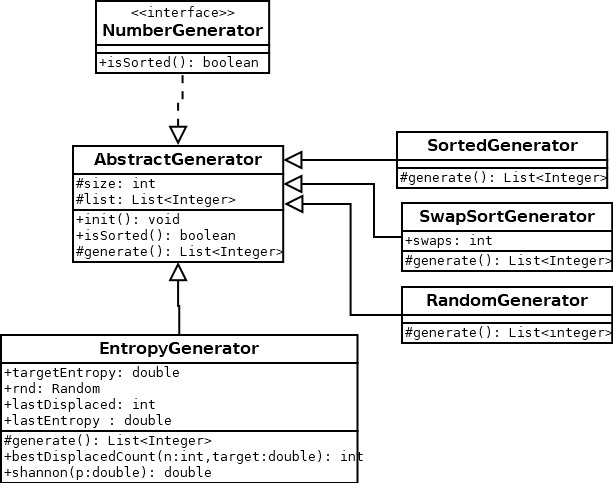
\includegraphics[width=\linewidth]{generator.png}
        \caption{UML for generator}
        \label{fig:gen1}
    \end{subfigure}
    \hfill
    \begin{subfigure}{0.35\textwidth}
        \centering
        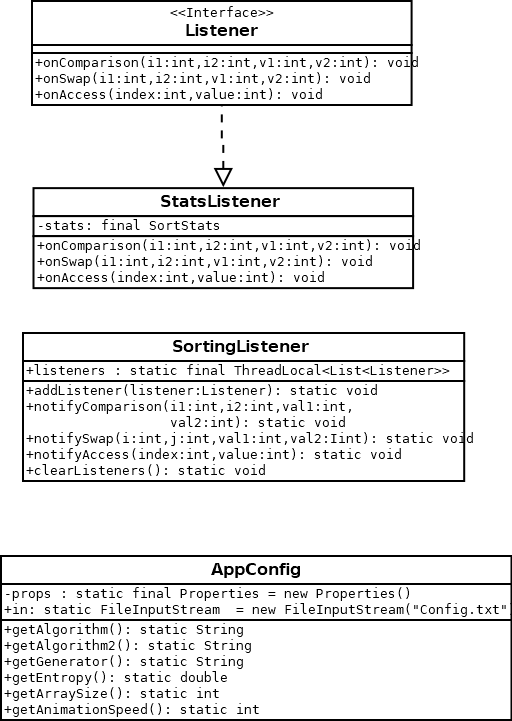
\includegraphics[width=\linewidth]{util.png}
        \caption{UML for util}
        \label{fig:sort}
    \end{subfigure}
    \caption{UML diagrams for the data generation and utility packages. 
The generator hierarchy is built around \texttt{NumberGenerator} and 
\texttt{AbstractGenerator}, while the util package shows the listener 
system and \texttt{AppConfig}.}
    \label{fig:uml}
\end{figure}


The \texttt{sorting} diagram presents the implemented algorithms and the role of \texttt{SortingAlgorithmFactory} in providing a common access point to them. 
The \texttt{model} diagram is simpler, but it is still important because it isolates \texttt{SortStats}, which stores the collected metrics.

\begin{figure}[H]
    \centering

    \begin{subfigure}{0.7\textwidth}
        \centering
        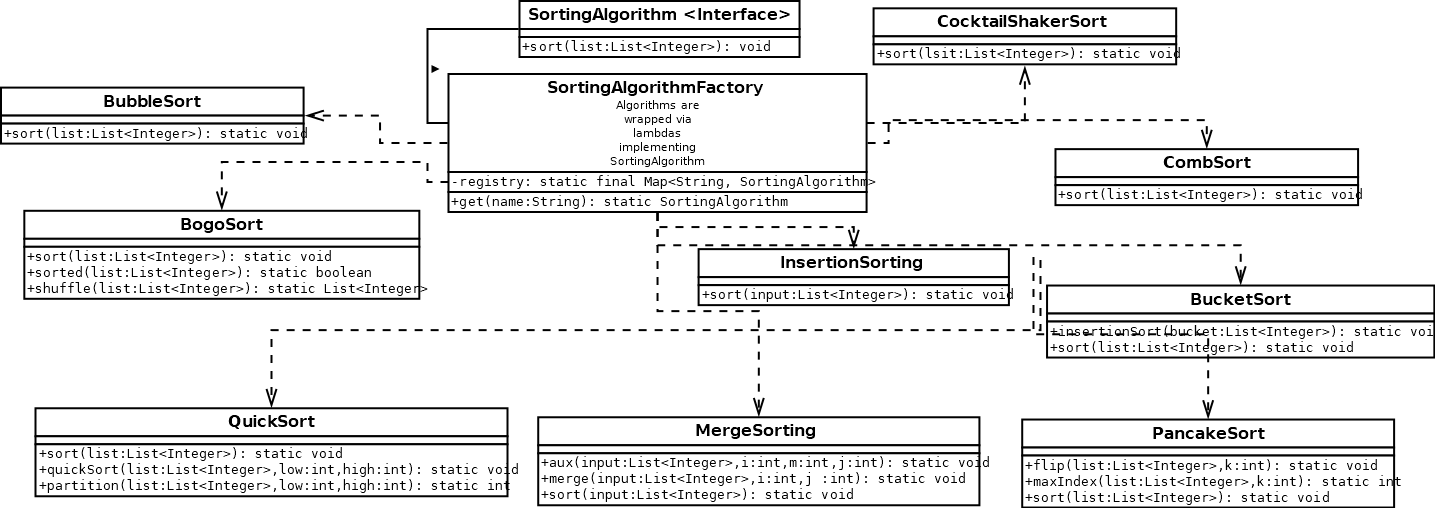
\includegraphics[width=\linewidth]{sorting.png}
        \caption{UML for sorting}
        \label{fig:gen2}
    \end{subfigure}
    \hfill
    \begin{subfigure}{0.2\textwidth}
        \centering
        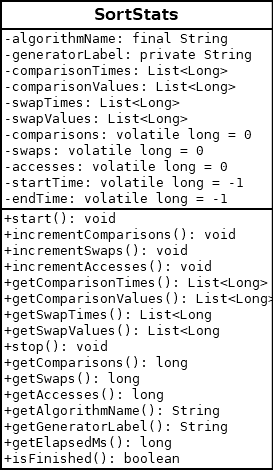
\includegraphics[width=\linewidth]{model.png}
        \caption{UML for model}
        \label{fig:sort1}
    \end{subfigure}

    \caption{UML diagrams for the sorting and model packages. 
\texttt{SortingAlgorithmFactory} provides a single access point to all 
algorithm implementations, and \texttt{SortStats} isolates the collected 
metrics.}
    \label{fig:uml1}
\end{figure}

The controller diagram is 
especially important because it shows how the controllers and sort runners connect 
the graphical interface to the algorithmic part of the application.
We also produced separate diagrams for the graphical structure. One for \texttt{view.menu}, one for \texttt{view.components}, and one for \texttt{view.windows}. This choice reflects the way we structured our interface. The 
menu diagram presents the entry points and user choices, the components diagram
focuses on graphical elements, and the windows diagram shows how the main 
screens of the application are organized around the abstract visualizer model.

\begin{figure}[H]
    \centering
    \begin{subfigure}{0.4\textwidth}
        \centering
        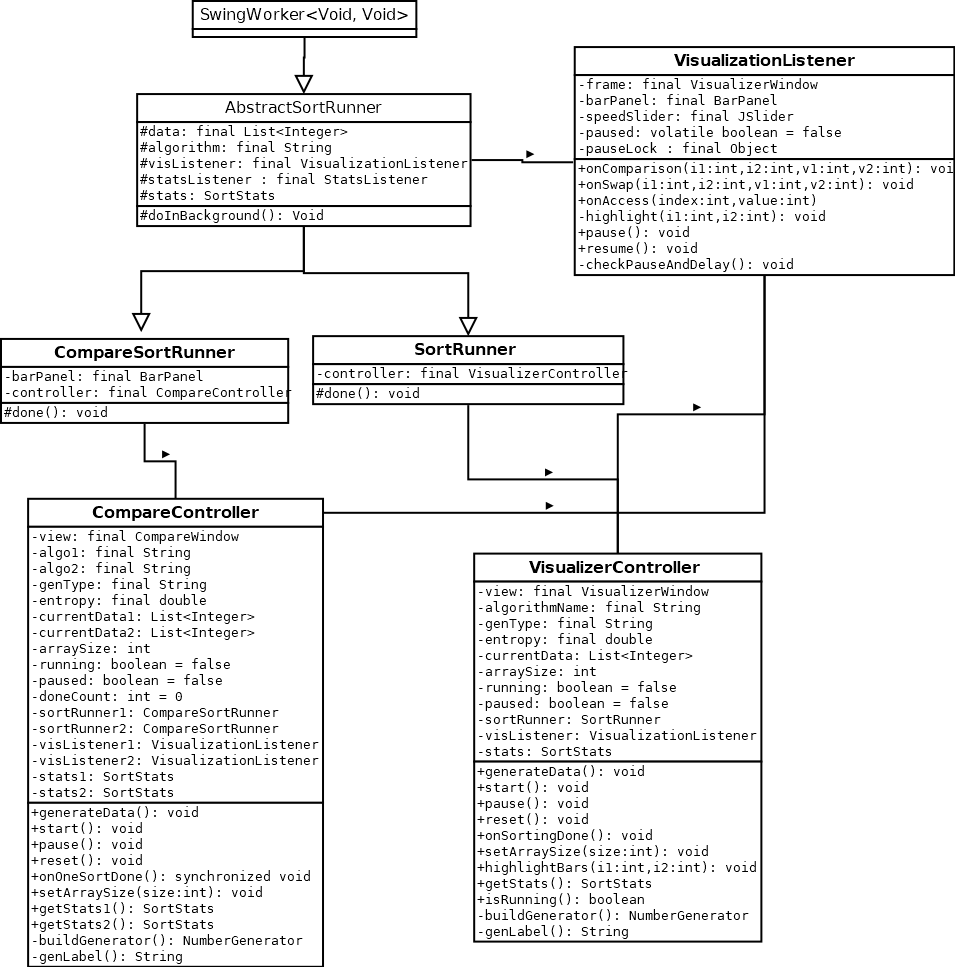
\includegraphics[width=\linewidth]{controller.png}
        \caption{UML for controller}
        \label{fig:img1}
    \end{subfigure}
    \hfill
    \begin{subfigure}{0.4\textwidth}
        \centering
        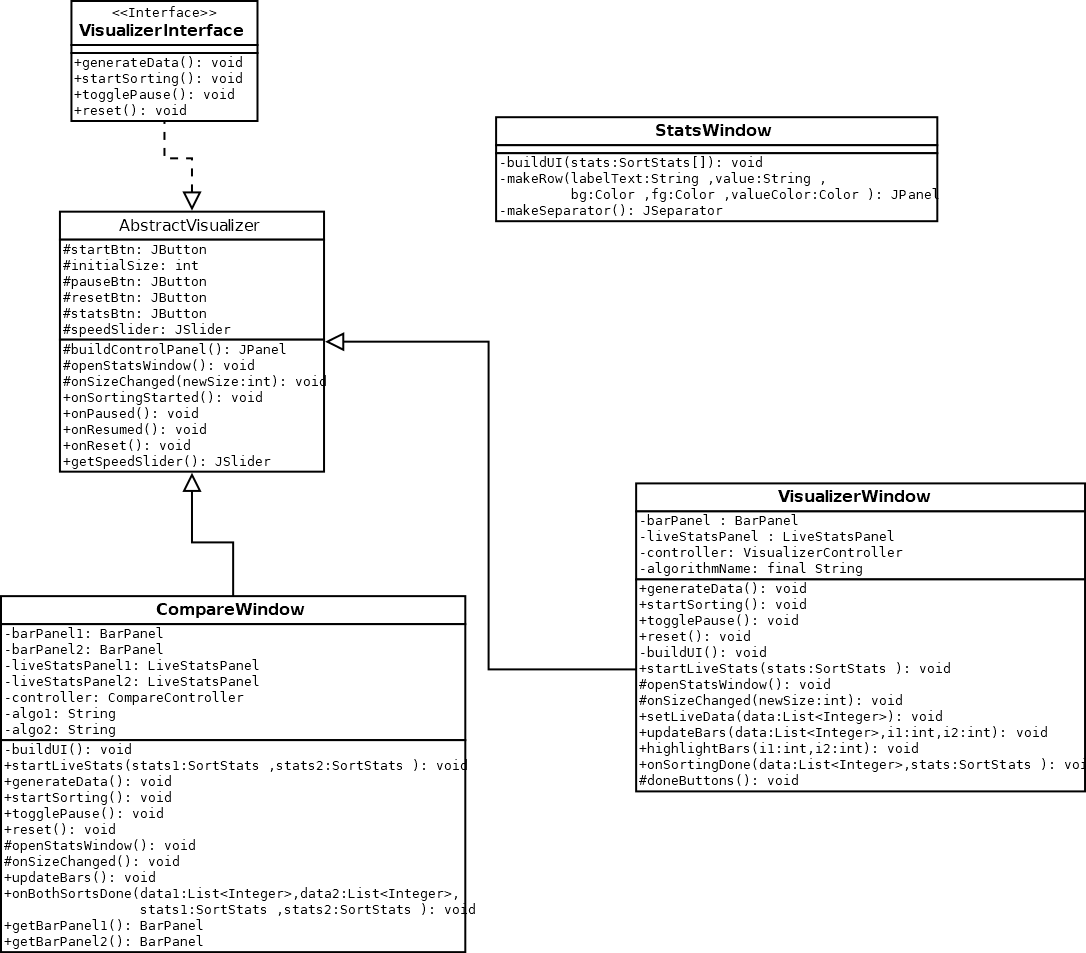
\includegraphics[width=\linewidth]{view_window.png}
        \caption{UML for view.window}
        \label{fig:img4}
    \end{subfigure}

    \vspace{0.5cm}

    \begin{subfigure}{0.45\textwidth}
        \centering
        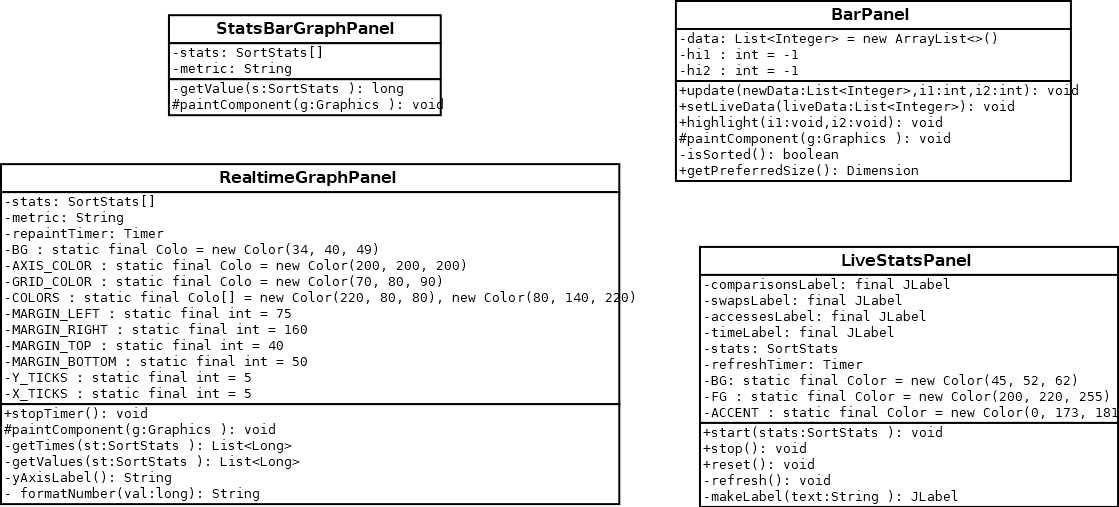
\includegraphics[width=\linewidth]{view_components.png}
        \caption{UML for view.components}
        \label{fig:img3}
    \end{subfigure}
    \hfill
    \begin{subfigure}{0.5\textwidth}
        \centering
        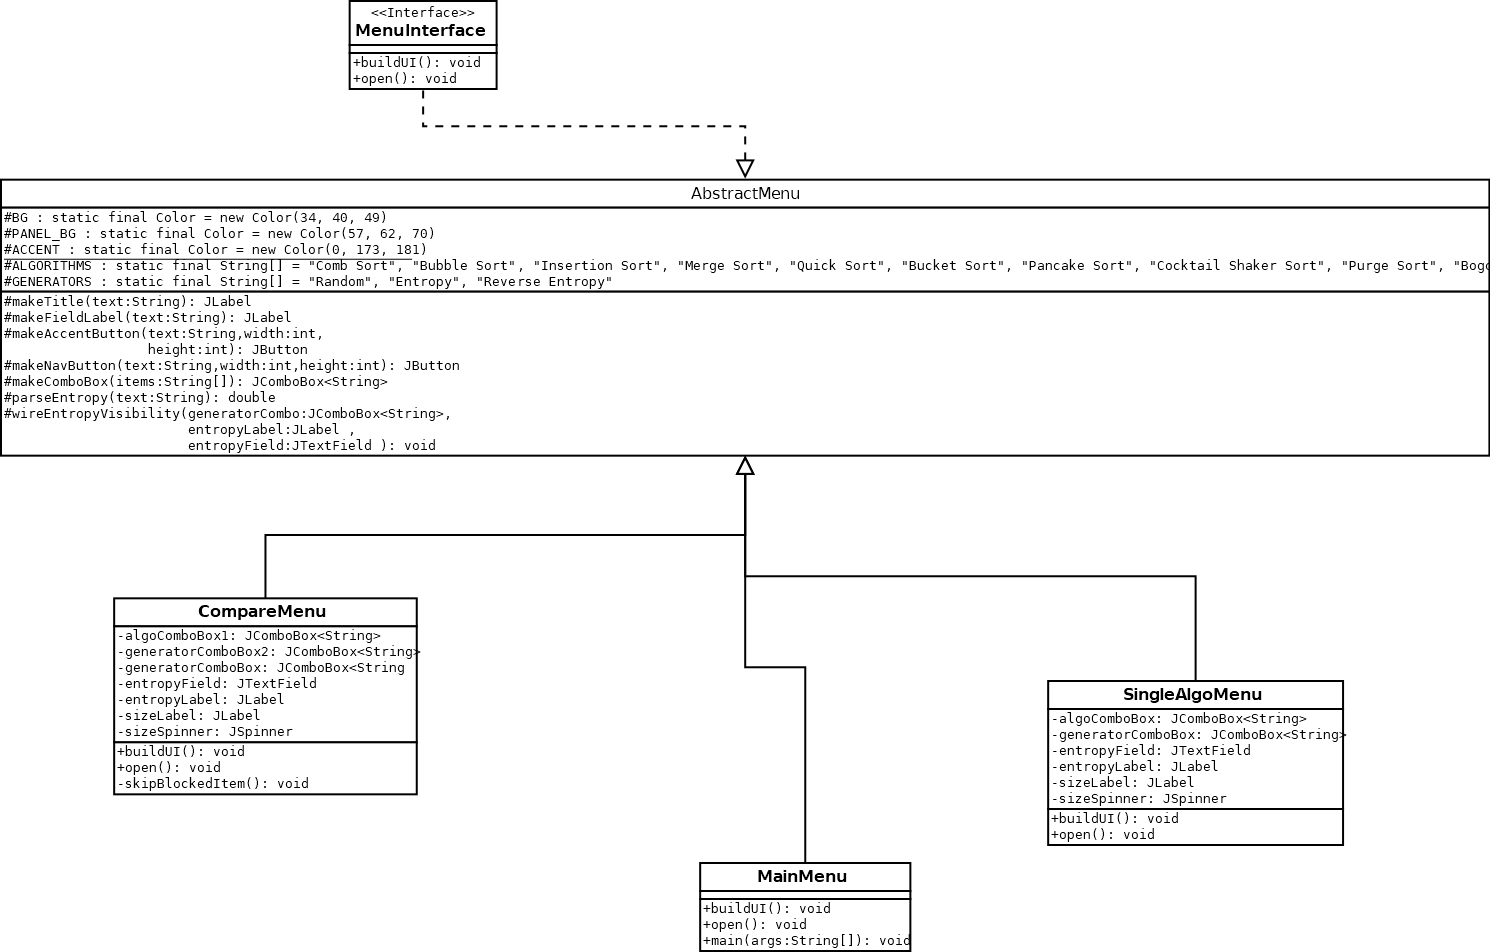
\includegraphics[width=\linewidth]{view_menu.png}
        \caption{UML for view.menu}
        \label{fig:img2}
    \end{subfigure}

    \caption{UML diagrams for the controller and view packages, showing how 
the execution logic connects to the graphical interface through the 
sort runner hierarchy and the visualizer windows.}
    \label{fig:all}
\end{figure}

Finally, we produced diagrams for the \texttt{benchmark} and \texttt{export} 
packages. These diagrams are simpler than the others, but they are important 
because they show that the experimentation pipeline is not mixed directly with the 
visualization logic. In other words, we separated interactive use from systematic 
benchmarking, which made the application easier to understand and extend.



\begin{figure}[H]
    \centering

    \begin{subfigure}{0.55\textwidth}
        \centering
        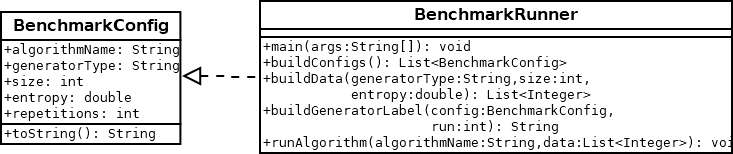
\includegraphics[width=\linewidth]{benchmark.png}
        \caption{UML for benchmark}
        \label{fig:gen}
    \end{subfigure}
    \hfill
    \begin{subfigure}{0.4\textwidth}
        \centering
        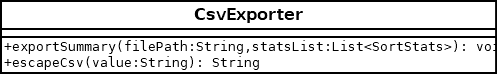
\includegraphics[width=\linewidth]{export.png}
        \caption{UML for export}
        \label{fig:sort2}
    \end{subfigure}
    \caption{UML diagrams for the benchmark and export packages, showing 
the separation between the systematic experimentation pipeline and the 
interactive visualization logic.}
    \label{fig:uml2}
\end{figure}



Overall, these diagrams confirm the modular structure of our application. Instead of 
building a messy and unorganized  project, we organized our work into specialized 
modules that communicate through well-defined responsibilities. This is one of the 
reasons why it was possible for us to add new algorithms, new graphs, or new 
benchmark features progressively during the project without needing to rewrite the 
whole codebase.

\subsection{Processing interactions: how the classes interact and why}
Our architecture follows a clear execution depending on the feature being used. The
first interaction is the single-algorithm visualization mode. The user starts from \texttt{MainMenu}, then opens \texttt{SingleAlgoMenu}, where an algorithm, a 
generator, an entropy value, and a list size can be selected. After validation, a \texttt{VisualizerWindow} is created. This window delegates the execution logic to \texttt{VisualizerController}, which generates the data through the appropriate class
from the \texttt{generator} package and sends this data to the graphical 
components.
When the user starts the execution, the controller creates a \texttt{SortRunner}, 
which extends \texttt{AbstractSortRunner}. This runner registers two listeners 
before launching the selected algorithm, such as a \texttt{VisualizationListener}, 
which updates the graphical bars during execution, and a \texttt{StatsListener}, 
which records comparisons, swaps, and accesses into a \texttt{SortStats} object. 
The sorting algorithm itself is retrieved through \texttt{SortingAlgorithmFactory}, 
which allows the controller to stay independent from the concrete implementation 
of each sort. This is important because it keeps the graphical layer, the control 
logic, and the algorithmic logic separated.
The second interaction is the comparison mode. From \texttt{MainMenu}, the user 
opens \texttt{CompareMenu}, chooses two different algorithms and one input 
configuration, then launches a \texttt{CompareWindow}. The \texttt{CompareController} generates one original list and copies it into two 
identical lists so that the comparison remains fair. It then starts two \texttt{CompareSortRunner} instances in parallel, one for each algorithm. Each 
runner has its own \texttt{VisualizationListener}, its own \texttt{StatsListener}, and
its own \texttt{SortStats} object. This is why the use of \texttt{ThreadLocal} in \texttt{SortingListener} is important, because it prevents the events of one 
algorithm from being mixed with the events of the other one during simultaneous 
execution.
The third interaction is the benchmarking and export workflow. In this case, the 
execution does not go through the graphical interface. Instead, \texttt{BenchmarkRunner} creates a series of \texttt{BenchmarkConfig} objects, 
builds the corresponding datasets through the generator classes, runs the 
algorithms, collects the statistics in \texttt{SortStats}, and finally passes the results
to \texttt{CsvExporter}. This architecture allowed us to keep experimental runs 
independent from the user interface while still reusing the same generators, 
algorithms, and statistics model.
A final interaction point is configuration. With \texttt{AppConfig}, we added a 
centralized way to load default values from \texttt{Config.txt}. This avoids 
hardcoding all startup parameters directly inside the menus or windows and makes 
our application easier to adjust without modifying the source code. Even though this
is a relatively small class compared to the rest of the architecture, it improves the 
overall maintainability of the application.
In summary, the interactions between our classes are clear and well organized. The 
menus collect the user choices, the windows display the corresponding screens, the 
controllers manage the execution logic, the runners launch the algorithms in the 
background, the listeners transmit the runtime events, the model stores the 
metrics, and the benchmark/export classes handle the large-scale experiments. We 
chose this architecture because it makes each responsibility explicit and keeps our 
application extensible, testable, and easier to understand.
\subsection{Design patterns used}
During the development of our application, we used several design patterns in order
to keep the code modular, reusable, and easier to extend. We added these patterns 
to help us structure the project more clearly and avoid strong coupling between the 
different parts of the application.
The first important pattern in our project is the \texttt{MVC} pattern. We separated 
our application into a graphical part, a control part, and a data part. The \texttt{view} packages contain the menus, windows, and graphical components. 
The \texttt{controller} package manages the execution flow and user actions. The \texttt{model} package contains \texttt{SortStats}, which stores the measured 
statistics. This separation was useful because it allowed us to modify the interface 
and the execution logic more independently.
Another important pattern is the \texttt{Observer} pattern. We used it through the 
listener system, especially with \texttt{Listener}, \texttt{SortingListener}, \texttt{StatsListener}, and \texttt{VisualizationListener}. During the execution of a 
sort, the algorithms notify events such as comparisons, swaps, and data accesses. 
These events are then received by the listeners, which either update the graphical 
interface or record statistics. We used this pattern because it lets us track the 
execution of the algorithms without hardcoding the visualization or statistics logic 
directly inside each sorting class.
We also used the \texttt{Strategy} pattern. In our project, the sorting algorithms 
and the data generators are behaviors selected at runtime. For example, different 
sorting algorithms can be accessed through the \texttt{SortingAlgorithm} 
abstraction, and different generators follow the same generation logic through the 
generator hierarchy. This pattern was useful because it allowed us to switch easily 
from one algorithm or generator to another without changing the rest of the 
application.
Closely related to this, we used a \texttt{Factory} pattern with \texttt{SortingAlgorithmFactory}. Instead of creating the sorting algorithms 
manually in several places, we centralized their selection inside one dedicated 
class. This made the code cleaner and avoided repeating large condition blocks 
each time we wanted to retrieve an algorithm from its name. It also made it easier 
for us to add new algorithms progressively during the project.
Finally, we used the \texttt{Template Method} pattern in the sort runner hierarchy. 
The class \texttt{AbstractSortRunner} defines a common structure for the 
execution of a sort, while subclasses such as \texttt{SortRunner} and 
\texttt{CompareSortRunner} specialize this behavior depending on the context. This
helped us avoid duplicating the common execution logic while still supporting both 
the single visualization mode and the compare mode.
Overall, these patterns allowed us to separate responsibilities, reuse common 
behaviors, and progressively enrich our application without needing to redesign the 
whole project each time we added a new feature

\section{Experimentations}
\label{sec:experiments}

\subsection{Use Cases}

\subsubsection{Benchmark Execution}

A first use case of the project is the execution of automated benchmarks on multiple sorting algorithms. The user launches the \texttt{BenchmarkRunner}, which iterates over a predefined set of benchmark configurations. Each configuration specifies:
\begin{itemize}
    \item the sorting algorithms,
    \item the generator type (\texttt{random}, \texttt{entropy}, or \texttt{reverse\_entropy}),
    \item the input size,
    \item the entropy level,
    \item the number of repetitions.
\end{itemize}

For each configuration, the system generates an input list, runs the selected sorting algorithms and records metrics such as comparisons, swaps, memory accesses, and execution time.

\subsubsection{Export of Experimental Results}

A second use case is the export of benchmark results for later analysis. After execution, the collected statistics are written to CSV files. These files can then be used to compare algorithms, compute averages, and prepare the quantitative analysis presented in this report.

Figure~\ref{fig:results-folder} shows a portion of a generated CSV file

\begin{figure}[h]
    \centering
    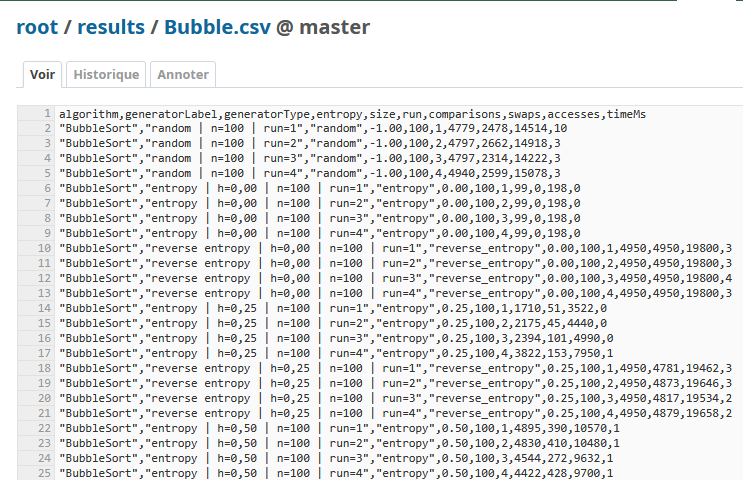
\includegraphics[width=0.8\textwidth]{results-folder.png}
    \caption{Example of a generated CSV result file using only BubbleSort.}
    \label{fig:results-folder}
\end{figure}

\subsubsection{Visualization and Comparison Mode}

Figure~\ref{fig:compare-viz} shows the compare mode during execution. 
Both algorithms run simultaneously on the same input (size 70, entropy 0.7). 
The red bars highlight the elements currently being accessed. The live 
statistics at the bottom of each panel are updated in real time, showing 
the number of comparisons, swaps, accesses, and elapsed time for each 
algorithm independently.

\begin{figure}[H]
    \centering
    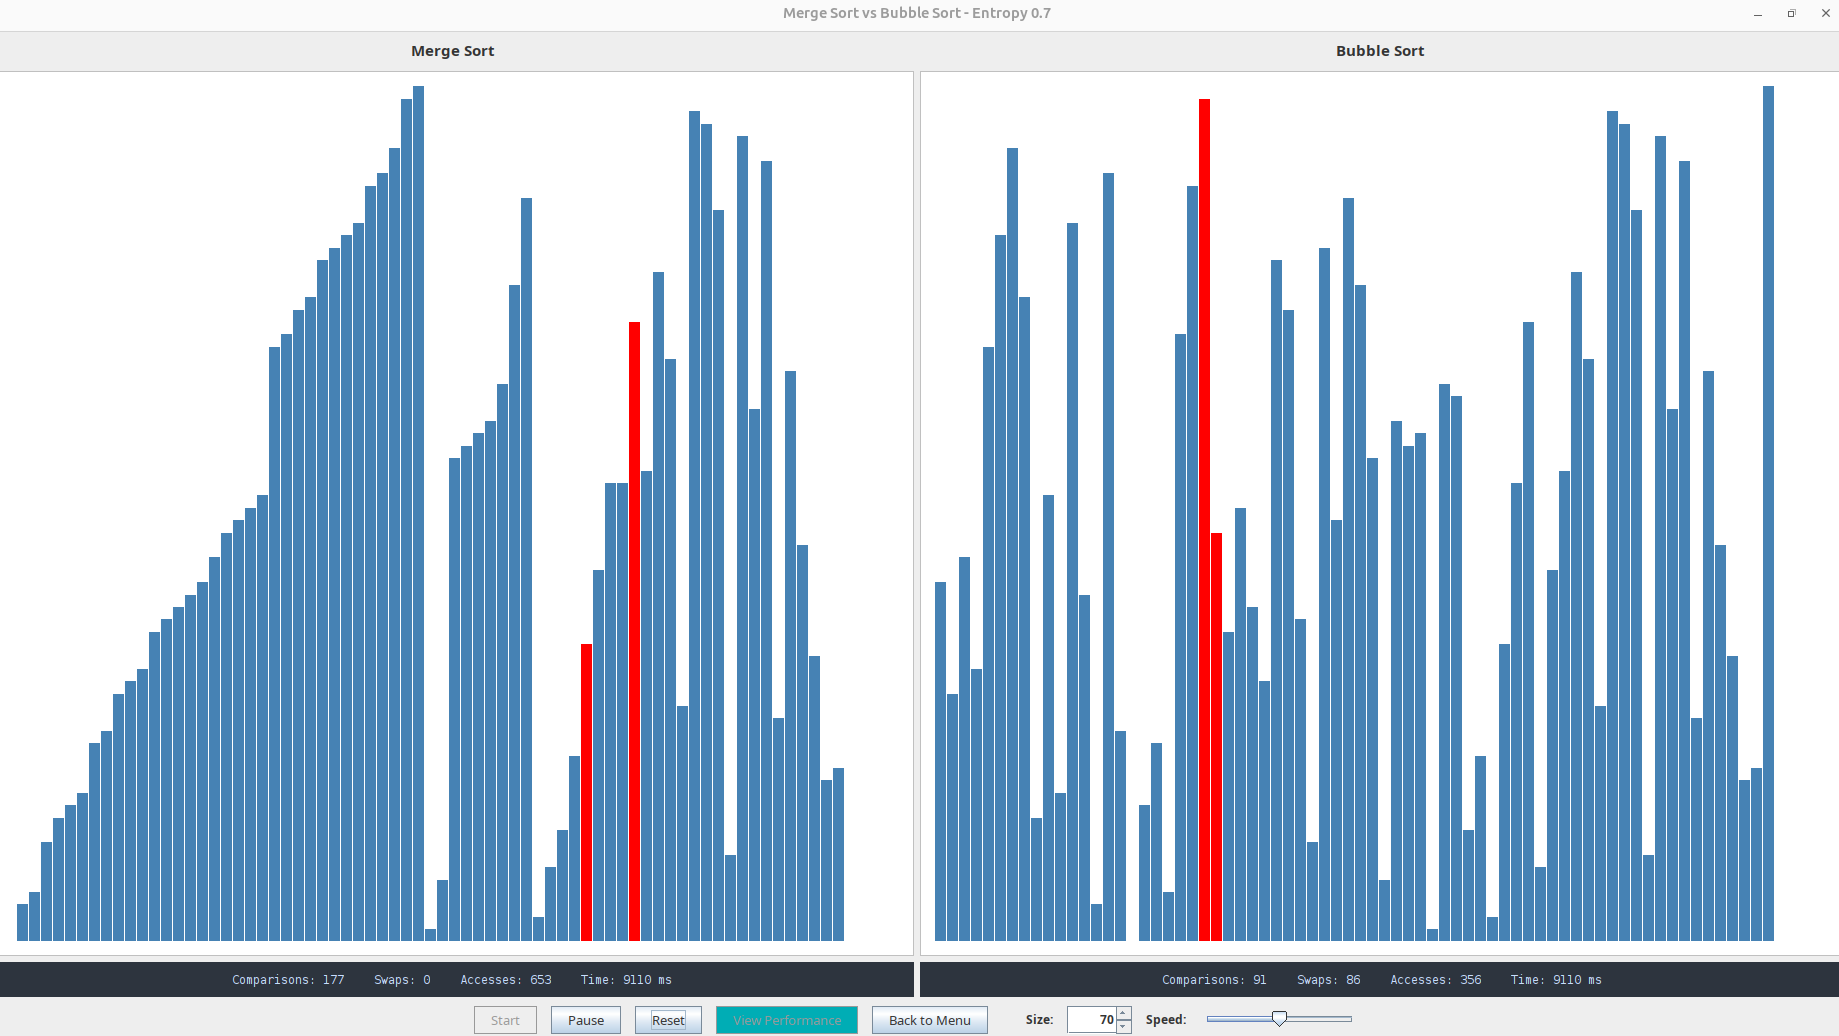
\includegraphics[width=0.9\textwidth]{ss1.png}
    \caption{Compare mode: Merge Sort (left) vs Bubble Sort (right) on an 
entropy 0.7 input of size 70, captured mid-execution. The left panel 
already shows large sorted regions forming, characteristic of Merge 
Sort's divide-and-conquer approach, while the right panel still shows 
high disorder, reflecting Bubble Sort's slow local propagation. The red 
bars indicate the elements currently being accessed in each algorithm.}
    \label{fig:compare-viz}
\end{figure}

Once both algorithms have finished, the user can open the Performance 
Statistics window (Figure~\ref{fig:compare-stats}), which displays the 
final metrics side by side. The graphs show the cumulative evolution of 
comparisons and swaps over time, while the bar charts at the bottom 
compare total execution time and memory accesses directly.

\begin{figure}[H]
    \centering
    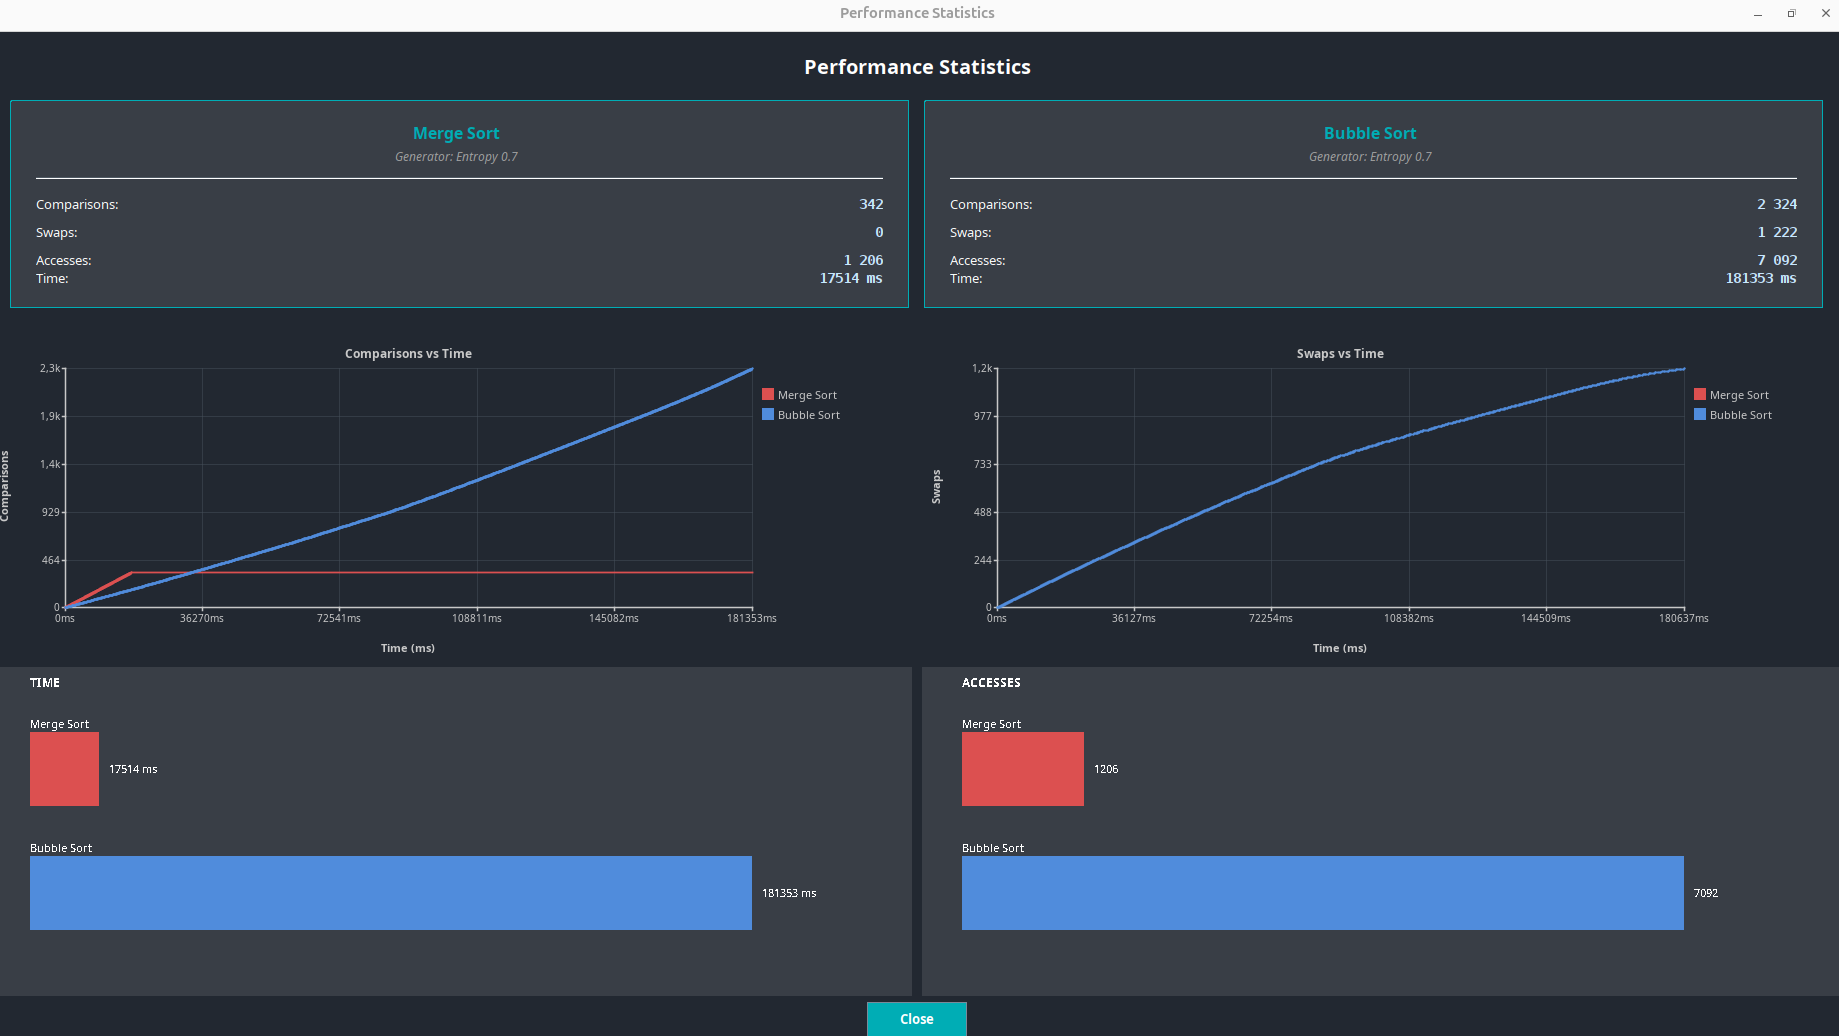
\includegraphics[width=0.9\textwidth]{ss2.png}
    \caption{Performance Statistics window after completion of Merge Sort 
    vs Bubble Sort on an entropy 0.7 input. Merge Sort completed in 
    17\,514\,ms with only 342 comparisons, while Bubble Sort required 
    181\,353\,ms and 2\,324 comparisons - roughly $6.8\times$ more time 
    and $6.8\times$ more comparisons.}
    \label{fig:compare-stats}
\end{figure}

\subsection{Quantitative Results and Analysis}

To evaluate the behavior of the sorting algorithms, each configuration was executed four times in order to reduce randomness and obtain more stable measurements.

Input lists were generated using different strategies: fully random data, entropy-controlled data, and reverse-entropy data. The entropy parameter $h \in [0,1]$ controls the structure of the generated list through a displacement-based entropy model, where $h=0$ corresponds to a sorted list and higher values are mapped by the generator to increasingly displaced configurations.

Experiments were conducted on multiple input sizes (100, 500, and 1000 elements). For each run, several metrics were collected, including the number of comparisons, swaps, memory accesses, and execution time.

\subsubsection{Random Input (Average Case)}

For the random input, the first run for $n=100$ was consistently higher across all algorithms. This behavior is not algorithm-specific and is likely caused by execution environment overhead. Therefore, these first runs are excluded from the analysis.

Under random input, most algorithms show their average-case behavior.

BubbleSort shows its quadratic growth. Comparisons increase from about 4800 ($n=100$) to $\sim 124500$ ($n=500$) and $\sim 498000$ ($n=1000$). Execution time rises from $\sim 3$ ms to 21--32 ms, then 85--134 ms. This confirms its $O(n^2)$ complexity, with no benefit from input structure.

CocktailShakerSort behaves similarly but slightly more efficient. Comparisons grow from $\sim 3800$--4000 to $\sim 93000$--99000, then $\sim 371000$--384000. Time increases from $\sim 2$--3 ms to 20--34 ms, then 77--86 ms. It remains quadratic but somewhat better than BubbleSort.

InsertionSort also follows quadratic growth. Comparisons increase from $\sim 2500$ to $\sim 61000$--65000, then $\sim 247000$--258000. Execution time rises from $\sim 2$--3 ms to 13--26 ms, then 59--85 ms. It performs slightly better than BubbleSort but still scales poorly.

MergeSort remains stable and efficient. Comparisons increase from $\sim 540$ ($n=100$) to $\sim 3850$ ($n=500$) and $\sim 8700$ ($n=1000$), consistent with $O(n \log n)$. Execution time stays very low: $\sim 1$ ms, $\sim 1$ ms, then $\sim 2$ ms. Its performance is unaffected by randomness.

QuickSort performs well and close to its expected average case. Comparisons grow from $\sim 600$--700 to $\sim 4500$--5000, then $\sim 10600$--11900, matching $O(n \log n)$. Execution time remains very low: $\sim 1$ ms for $n=100,500$ and 2--3 ms for $n=1000$. This confirms efficient pivot behavior on random data.

CombSort also performs efficiently. Comparisons increase from $\sim 1200$--1400 to $\sim 9300$--10300, then $\sim 21700$--23700. Execution time remains low: 1--2 ms, 2--5 ms, then 3--4 ms. It scales much better than its ancestor BubbleSort and other quadratic algorithms.

PancakeSort is the most inefficient of the bunch. Comparisons are fixed at 5148, 125748, and 501498, while time increases from $\sim 2$ ms to 28--43 ms, then 103--154 ms. Its behavior is clearly worse than both $O(n \log n)$ and optimized quadratic algorithms.

\subsubsection{Sorted Input (Entropy = 0)}

For $h=0$, the list is already sorted, so adaptive algorithms (Adaptive sorting algorithms exploit existing order in the input, reducing their complexity when the data is nearly sorted.) perform best.

BubbleSort, CocktailShakerSort, and InsertionSort all show the same pattern: for $n=100,500,1000$, they use exactly $n-1$ comparisons, 0 swaps, and their execution time stays at 0 or 1 ms. This confirms their best-case behavior on sorted data.

MergeSort also remains efficient but unlike the adaptive algorithms, it still performs more work even on sorted input. Its comparisons increase from 356 ($n=100$) to 2272 ($n=500$) and 5044 ($n=1000$), with times remaining very low (0 to 2 ms). This shows that MergeSort is stable but not adaptive to sortedness.

CombSort performs no swaps but still requires a significant number of comparisons (1003, 8372, 18713 for $n=100,500,1000$). Execution time remains low and stable across runs, indicating that the algorithm does not significantly benefit from sorted input.

QuickSort shows the opposite behavior. It clearly degrades as the input size increases: comparisons go from 4950 ($n=100$) to 124750 ($n=500$) and 499500 ($n=1000$), while execution time rises from about 2--3 ms to 38--81 ms and then 120--156 ms. This is its worst case, caused by always choosing the last element as pivot.

PancakeSort is also insensitive to sortedness. Its comparisons are very high even for sorted input: 5148, 125748, and 501498, with time increasing from 1 ms to 12 ms and then 54--99 ms. Its behavior is therefore much less favorable than the adaptive algorithms.


\subsubsection{Low Entropy Input ($H = 0.25$)}

At this target entropy level, the generated list remains close to sorted, so adaptive algorithms start to lose their best-case advantage, but they still remain more efficient than the non-adaptive algorithms.

BubbleSort is already strongly affected by this small disorder. Its comparisons increase from about 1.7k--3.8k at $n=100$ to about 112k--124k at $n=500$, then to about 437k--496k at $n=1000$. Execution time follows the same trend, from 0--1 ms to 13--15 ms, then 55--61 ms. This behavior is consistent with its quadratic complexity, $O(n^2)$.

CocktailShakerSort also degrades, but less severely than BubbleSort. Comparisons rise from about 295--487 at $n=100$ to 6.4k--7.4k at $n=500$, then 20.8k--24.7k at $n=1000$. Time increases from 0--1 ms to 1 ms, then 4--5 ms. It remains quadratic in the worst case, but its bidirectional passes make it much more effective on slightly disordered data.

InsertionSort remains one of the best-performing algorithms in this case. Comparisons increase from about 152--238 at $n=100$ to 3.0k--4.4k at $n=500$, then 14.6k--15.6k at $n=1000$. Execution time stays very low: 0--1 ms at $n=100$, 1 ms at $n=500$, and 4 ms at $n=1000$. This confirms that although its worst-case complexity is $O(n^2)$, it remains very efficient on nearly sorted data.

MergeSort stays stable, as expected from its $O(n \log n)$ complexity. Comparisons rise regularly from about 412--436 at $n=100$ to 3.0k--3.2k at $n=500$, then 6.7k--7.2k at $n=1000$. Time remains almost unchanged, from 0--1 ms to 0--1 ms, then 2 ms. Its performance is therefore not significantly affected by this low entropy.

CombSort shows moderate growth. Comparisons increase from 1201 at $n=100$ to about 8.9k--9.4k at $n=500$, then 21.7k at $n=1000$. Execution time remains low, from 0--1 ms to 1--2 ms, then 2--3 ms. Although it is not adaptive, it handles partial disorder much better than BubbleSort.

QuickSort improves a lot compared with $H=0$, but its results remain unstable. Comparisons go from about 2.2k--3.6k at $n=100$ to 24.9k--32.3k at $n=500$, then 32.1k--95.2k at $n=1000$. Execution time rises from 0--1 ms to 3--7 ms, then 4--15 ms. On average, this is much better than its worst case, but the variation between runs shows that pivot choice still has a strong effect.

PancakeSort remains largely insensitive to this lower entropy. Its comparisons are fixed at 5148 for $n=100$, 125748 for $n=500$, and 501498 for $n=1000$, with times increasing from 1 ms to 16 ms, then 61--66 ms. This reflects its rigid quadratic behavior and poor practical efficiency.

\subsubsection{Medium Entropy Input ($H = 0.5$)}

At this target entropy level, the generated input contains a substantial number of displaced elements, and most algorithms approach their average-case behavior.

BubbleSort clearly reaches its typical quadratic behavior. Comparisons increase from about 4.4k--4.9k at $n=100$ to 116k--124k at $n=500$, then 490k--498k at $n=1000$. Execution time rises sharply from 1 ms to 12--35 ms, then up to 53--148 ms. This confirms $O(n^2)$ growth with no remaining benefit from partial order.

CocktailShakerSort follows a similar trend but remains more efficient. Comparisons grow from 675--859 ($n=100$) to 15k--16k ($n=500$), then 55k--66k ($n=1000$). Execution time increases from 0--1 ms to 2--3 ms, then 12--14 ms. It still outperforms BubbleSort but behaves quadratically.

InsertionSort is now much more affected by disorder. Comparisons increase from 417--625 at $n=100$ to 9.5k--11.4k at $n=500$, then 34k--40k at $n=1000$. Execution time rises from 0--1 ms to 2--3 ms, then 6--10 ms (with one outlier). This reflects its transition toward $O(n^2)$ as the level of displacement increases.

MergeSort remains stable and unaffected. Comparisons scale regularly from 423--469 at $n=100$ to 3.3k--3.4k at $n=500$, then 7.5k--7.9k at $n=1000$. Execution time stays nearly constant (0--2 ms), confirming its $O(n \log n)$ behavior regardless of input.

CombSort shows moderate degradation. Comparisons increase from 1201 ($n=100$) to 8.8k--9.3k ($n=500$), then 21.7k--23.7k ($n=1000$). Execution time grows slightly (0--1 ms $\rightarrow$ 1--2 ms $\rightarrow$ 2--3 ms). It is not adaptive but remains efficient in practice.

QuickSort performs much better than in low-entropy or sorted cases. Comparisons grow from 1.1k--2.2k at $n=100$ to 6.4k--16.3k at $n=500$, then 19.7k--46.5k at $n=1000$. Execution time stays low (0 ms $\rightarrow$ 1--2 ms $\rightarrow$ 2--7 ms). This is close to its expected average-case $O(n \log n)$, though variability between runs remains due to pivot choice.

PancakeSort continues to show strictly quadratic behavior. Comparisons are fixed at 5148, 125748, and 501498, with execution time increasing from 1 ms to 14--15 ms, then 63--111 ms.


\subsubsection{High Entropy Input ($H = 0.75$)}

At this target entropy level, the generated list contains a high proportion of displaced elements, so most algorithms behave close to their average-case behavior.

BubbleSort is now fully in its quadratic form. Comparisons increase from about 4.8k--4.9k at $n=100$ to about 123.9k--124.7k at $n=500$, then 498.9k--499.4k at $n=1000$. Execution time rises from 1 ms to 22--24 ms, then 69--129 ms. This confirms that the high level of displacement removes any advantage from partial order.

CocktailShakerSort shows the same general trend. Comparisons grow from about 3.1k--3.4k at $n=100$ to 72.8k--87.2k at $n=500$, then 309.7k--330.1k at $n=1000$. Time increases from 1 ms to 13--15 ms, then 54--113 ms. It remains better than BubbleSort, but still clearly quadratic.

InsertionSort also loses most of its adaptiveness at this entropy level. Comparisons rise from about 2.2k--2.4k at $n=100$ to 51.1k--55.9k at $n=500$, then 214.3k--219.5k at $n=1000$. Execution time grows from 0--1 ms to 9--26 ms, then 43--120 ms. This shows that with a high level of displacement, its $O(n^2)$ behavior becomes much more visible.

MergeSort remains stable, as expected. Comparisons increase regularly from 536--552 at $n=100$ to 3836--3863 at $n=500$, then 8674--8714 at $n=1000$. Execution time stays very low, from 0--1 ms to 0--1 ms, then 2 ms. Its $O(n \log n)$ behavior is unchanged by the higher entropy.

CombSort is only moderately affected. Comparisons increase from about 1201--1300 at $n=100$ to 8.9k--9.9k at $n=500$, then 21.7k--23.7k at $n=1000$. Execution time remains low: 0--1 ms, then 1--2 ms, then 2--3 ms. It is not adaptive, but it remains efficient even on highly displaced input.

QuickSort performs very well in this case. Comparisons grow from about 640--684 at $n=100$ to 4380--5671 at $n=500$, then 10.5k--12.4k at $n=1000$. Execution time stays extremely low, from 0--1 ms to 0--1 ms, then 1--2 ms. This is close to its expected average-case $O(n \log n)$, and the results are also much more stable than for lower entropy.

PancakeSort remains strictly quadratic and insensitive to structure. Comparisons are fixed at 5148, 125748, and 501498 for $n=100,500,1000$, while execution time increases from 1--2 ms to 26--46 ms, then 110--148 ms. It remains one of the least efficient algorithms in practice.


\subsubsection{Reverse Sorted Input (Reverse Entropy, $H = 0$)}

This case corresponds to the maximum order in the opposite direction: the list is fully reverse sorted. It is a worst-case configuration for several quadratic algorithms.

BubbleSort reaches its worst case here. Comparisons and swaps are exactly identical: 4950 at $n=100$, 124750 at $n=500$, and 499500 at $n=1000$. Execution time increases from 3--4 ms to 25--57 ms, then 111--172 ms. This is consistent with its quadratic $O(n^2)$ behavior.

CocktailShakerSort behaves similarly. Comparisons grow from 5000 to 125000 and 500000, while swaps are 4950, 124750, and 499500. Time rises from 3--4 ms to 25--58 ms, then 115--164 ms. Its bidirectional passes do not help in this extreme case.

InsertionSort also reaches its worst case. Comparisons and swaps are again 4950, 124750, and 499500, with times increasing from 3--4 ms to 24--46 ms, then 117--153 ms. This confirms its quadratic cost on reverse-ordered input.

MergeSort remains stable and efficient. Comparisons increase regularly from 316 at $n=100$ to 2216 at $n=500$, then 4932 at $n=1000$, while execution time stays at 0--1 ms. As in the previous cases, its $O(n \log n)$ complexity is unaffected by input order.

CombSort handles reverse order much better than the quadratic neighboring-swap algorithms. Comparisons increase from 1102 to 8871 and 19712, with swaps only 122, 730, and 1582. Execution time remains very low, around 0--2 ms. This shows that CombSort is much less sensitive to reverse order.

QuickSort again reaches a worst-case situation in terms of comparisons: 4950, 124750, and 499500. However, its swap count is lower than for sorted input (2549, 62749, 250499), since the pivot is always the smallest element and partitions are still maximally unbalanced. Execution time rises from 1--2 ms to 17--46 ms, then 78--137 ms. This confirms that with last-element pivot selection, reverse-sorted input is also a worst case.

PancakeSort remains quadratic in comparisons, with fixed values 5148, 125748, and 501498, but performs very few swaps in this case: only 50, 250, and 500. Execution time still increases significantly from 1 ms to 13--44 ms, then 48--92 ms. Its behavior is therefore still inefficient, even if the number of flips is low.


\subsubsection{Reverse Low Entropy Input (Reverse Entropy, $H = 0.25$)}

At this reverse target entropy level, the generated input remains close to reverse sorted, so several quadratic algorithms are still near their worst case.

BubbleSort is barely improved compared with reverse $H=0$. Comparisons remain essentially maximal: 4950 at $n=100$, 124750 at $n=500$, and 499499--499500 at $n=1000$. Swaps are only slightly lower than in the fully reverse-sorted case, and execution time still rises strongly from 2--3 ms to 23--42 ms, then 107--191 ms. Its quadratic $O(n^2)$ behavior is therefore unchanged.

CocktailShakerSort behaves similarly. Comparisons stay near their maximum, from about 4992--4998 at $n=100$ to 124928--124968 at $n=500$, then 499712--499800 at $n=1000$. Time grows from 3 ms to 30--38 ms, then 106--153 ms. Like BubbleSort, it remains highly sensitive to reverse-ordered structure.

InsertionSort also stays close to its worst case. Comparisons increase from about 4844--4937 at $n=100$ to 120773--122059 at $n=500$, then 486026--487567 at $n=1000$. Execution time rises from 3 ms to 30--36 ms, then 106--173 ms. This confirms that a small amount of disorder does not significantly help InsertionSort when the base order is reversed.

MergeSort remains stable and efficient. Comparisons grow from 354--417 at $n=100$ to 2835--3192 at $n=500$, then 6799--7097 at $n=1000$, while execution time stays at 0--1 ms and then 1--2 ms. Its $O(n \log n)$ behavior is again unaffected by the input structure.

CombSort continues to handle this case well. Comparisons rise from 1102--1201 at $n=100$ to 8871--9370 at $n=500$, then remain around 21710 at $n=1000$. Execution time stays very low, around 0--1 ms for small inputs and 2 ms at $n=1000$. This confirms that CombSort is much less sensitive to reverse disorder than the quadratic neighboring-swap methods.

QuickSort improves a lot compared with reverse $H=0$, but remains unstable. Comparisons increase from about 1825--3211 at $n=100$ to 11892--32334 at $n=500$, then 28327--77895 at $n=1000$. Execution time grows from 0--1 ms to 2--6 ms, then 5--15 ms. This is much better than the pure reverse-sorted case.

PancakeSort remains structurally unchanged in comparisons, which are fixed at 5148, 125748, and 501498. Execution time increases from 1 ms to 13--26 ms, then 56--112 ms. Its performance is therefore still dominated by its rigid quadratic structure.

Overall, reverse $H=0.25$ still behaves much more like the reverse-sorted case than like the standard $H=0.25$ case. BubbleSort, CocktailShakerSort, and InsertionSort remain near worst-case performance, while MergeSort and CombSort stay efficient. QuickSort improves noticeably, but remains less stable than the other $O(n \log n)$-type behaviors.


\subsubsection{Reverse Medium Entropy Input (Reverse Entropy, $H = 0.5$)}

At this reverse target entropy level, the generated input is still strongly influenced by the reverse order, but the level of displacement is now high enough for some algorithms to improve compared with reverse $H=0$ and reverse $H=0.25$.

BubbleSort remains close to its worst case. Comparisons stay maximal or almost maximal: about 4950 at $n=100$, 124750 at $n=500$, and 499500 at $n=1000$. Swaps decrease slightly compared with the fully reverse-sorted case, but execution time still grows from 1--2 ms to 26--27 ms, then 120--137 ms. Its behavior is therefore still quadratic.

CocktailShakerSort shows the same pattern. Comparisons remain near maximum, from about 4968--4992 at $n=100$ to 124488--124712 at $n=500$, then 498078--499422 at $n=1000$. Time increases from 1--3 ms to 22--26 ms, then 106--165 ms. It remains heavily penalized by reverse-oriented data.

InsertionSort also stays near worst-case behavior. For $n=100$, comparisons are about 4561--4790, and for $n=500$, about 115567--116677, with execution times rising from 2--3 ms to 21--22 ms. Only one $n=1000$ result is visible in the provided data (465718 comparisons, 118 ms), but it is consistent with the same quadratic trend. So even at reverse $H=0.5$, InsertionSort remains very expensive.

MergeSort again remains stable and efficient. Comparisons increase regularly from 411--448 at $n=100$ to 3148--3339 at $n=500$, then 7593--7801 at $n=1000$. Execution time stays very low, from 0 ms to 0--1 ms, then 1--2 ms. Its $O(n \log n)$ behavior is unchanged.

CombSort continues to handle reverse entropy well. Comparisons increase from about 1102--1300 at $n=100$ to 8871--9370 at $n=500$, then 21710--22709 at $n=1000$. Execution time remains low: 0--1 ms, then 1--2 ms, then 3 ms. This confirms that CombSort is much less sensitive to reverse disorder than the quadratic algorithms.

QuickSort improves significantly compared with reverse $H=0$ and also becomes more stable than at reverse $H=0.25$. Comparisons rise from about 1075--3284 at $n=100$ to 6454--9461 at $n=500$, then 18787--27544 at $n=1000$. Execution time stays low, from 0--1 ms to 1--2 ms, then 3--4 ms. This is much closer to its expected average-case behavior.

PancakeSort remains rigid in comparisons, with fixed values 5148, 125748, and 501498 for $n=100,500,1000$. Execution time increases from 1 ms to 17 ms, then 68--83 ms. As before, it does not benefit much from the input structure.


\subsubsection{Reverse High Entropy Input (Reverse Entropy, $H = 0.75$)}

At this reverse target entropy level, the generated input is still influenced by the reverse order, but it is much more displaced than in the previous reverse cases. Several algorithms therefore move closer to their average-case behavior.

BubbleSort remains quadratic. Comparisons stay near their maximum: about 4872--4950 at $n=100$, 124254--124744 at $n=500$, and 499455--499500 at $n=1000$. Execution time increases from 1 ms to 25--28 ms, then 113--123 ms. The reverse structure is therefore still enough to keep BubbleSort very expensive.

CocktailShakerSort also remains costly. Comparisons rise from about 3942--4352 at $n=100$ to 103987--108619 at $n=500$, then 424339--436987 at $n=1000$. Time increases from 1--2 ms to 17--18 ms, then 75--121 ms. It is slightly better than BubbleSort, but still clearly quadratic.

InsertionSort continues to degrade strongly with size. Comparisons increase from about 3050--3121 at $n=100$ to 71767--73575 at $n=500$, then 288012--293442 at $n=1000$. Execution time rises from 1 ms to 12--13 ms, then around 61 ms in most runs. So even at reverse $H=0.75$, it remains much more expensive than the $O(n \log n)$ algorithms.

MergeSort again stays stable. Comparisons grow regularly from 524--544 at $n=100$ to 3808--3845 at $n=500$, then 8658--8699 at $n=1000$. Execution time remains very low, from 0--1 ms to 0--1 ms, then 2--3 ms. Its behavior is unchanged by reverse entropy.

CombSort remains efficient. Comparisons increase from about 1201--1300 at $n=100$ to 9370--9869 at $n=500$, then 21710--22709 at $n=1000$. Execution time stays low: 0--1 ms, then 2 ms, then 3 ms. This confirms that CombSort handles reverse disorder much better than the quadratic methods.

QuickSort performs very well in this case. Comparisons rise from about 606--703 at $n=100$ to 4646--5886 at $n=500$, then 10786--13121 at $n=1000$. Execution time stays extremely low, from 0 ms to 1 ms, then 1--2 ms. At this entropy level, it is close to its expected average-case $O(n \log n)$.

PancakeSort remains rigid in comparisons, with fixed values 5148, 125748, and 501498 for $n=100,500,1000$. Execution time increases from 1--2 ms to 28--29 ms, then 108--124 ms. It therefore remains inefficient despite the increased disorder.

Overall, reverse $H=0.75$ reduces the penalty of reverse-oriented input for some algorithms, especially QuickSort, while MergeSort and CombSort remain consistently efficient. In contrast, BubbleSort, CocktailShakerSort, and InsertionSort still show clear quadratic growth, and PancakeSort remains inefficient.



\subsection{Results Conclusion of the Analysis}

The experimental results clearly highlight that the behavior of sorting algorithms depends strongly on both input structure and algorithm design.

The first valuable observation appears between adaptive algorithms and input-insensitive algorithms. InsertionSort, BubbleSort, and CocktailShakerSort benefit significantly from low entropy (nearly sorted data), achieving very low costs at $H=0$. However, as the level of displacement increases or when the input is reverse-oriented their performance quickly worsens to their quadratic $O(n^2)$, making them inefficient for larger inputs.

In contrast, MergeSort demonstrates complete independence from input structure. Its performance remains stable across all entropy levels and input types, consistently following $O(n \log n)$. This makes it the most predictable and reliable algorithm in all scenarios.

QuickSort shows a different kind of sensitivity: it depends heavily on pivot selection and input structure. It performs poorly on sorted or reverse-sorted inputs (worst case), but becomes highly efficient and stable on random or high-entropy data, where it closely matches its average-case $O(n \log n)$.

CombSort can also be named as an improved BubbleSort. It introduces a gap that shrinks over time, eliminating small values near the end much faster than BubbleSort. As a result, it retains simplicity while significantly improving performance over BubbleSort. It is not adaptive, but it remains consistently efficient across all input types and avoids the extreme slowdowns of quadratic algorithms.

Finally, PancakeSort stands out as the least efficient algorithm. Its number of comparisons remains fixed regardless of input. As a result, it consistently shows poor performance compared to all other algorithms.

\paragraph{Which algorithm is best for which case}

\begin{itemize}
    \item Nearly sorted data (low entropy):\\
    $\rightarrow$ InsertionSort is the best choice due to its strong adaptiveness and very low overhead.

    \item Random or high-entropy data: \\
 $\rightarrow$ QuickSort performs best in practice, offering excellent speed with low constants. \\
 $\rightarrow$ MergeSort is a safer alternative if stability and consistency are required.

    \item Worst-case or unknown input: \\
 $\rightarrow$ MergeSort is the most reliable, as its performance is guaranteed regardless of input.

    \item Simple improvement over BubbleSort:\\
$\rightarrow$ CombSort is preferable, as it keeps a similar idea but avoids BubbleSort's inefficiency.

    \item ``At Least You Tried Award'':\\
$\rightarrow$ PancakeSort, due to its poor practical performance.
\end{itemize}

\paragraph{Overall ``winner'' ?}

If a single algorithm must be selected as the overall best, MergeSort can be named as the winner.

While QuickSort is often faster in favorable conditions, MergeSort provides:
\begin{itemize}
    \item consistently low execution time
    \item predictable $O(n \log n)$ complexity in all cases
    \item complete independence from input structure
\end{itemize}

This makes it the most consistent and reliable choice across all tested scenarios.

That said, in practical situations where input is random and performance is critical, QuickSort is often faster than MergeSort yet its performance is highly inefficient across its worst case conditions (up to $\sim 50\times$ slower in our experiments!).


\section{Conclusion}

\subsection{Summary of the problem and the achievement} 
This project set out to answer how the efficiency of sorting algorithms 
varies depending on the quantity and distribution of disorder in the 
input data. To answer this question, we built a complete pipeline 
combining a Shannon entropy-based data generator, nine instrumented 
sorting algorithms, a real-time visualization interface, and a 
systematic benchmark system. The detailed results and their analysis 
are presented in Section~\ref{sec:experiments}.

\subsection{Summary of the results}

Overall, the experiments confirm that no single sorting algorithm is optimal in every situation. Adaptive algorithms perform best on nearly sorted data, QuickSort is the fastest in favorable average-case conditions, and MergeSort stands out as the most reliable and consistent choice across all tested scenarios.

\subsection{Future improvements}

In the future, we can make a few improvements :
\begin{enumerate}
    \item The data generator could be extended to support lists with duplicate values, which would allow studying algorithm behavior under value collisions.
    
    \item The visualization could be improved by adding a step-by-step mode where the user can advance the sort one operation at a time.
    
    \item The project currently only supports comparison-based sorting algorithms. Adding non-comparison algorithms such as \texttt{Radix Sort} or \texttt{Counting Sort} would broaden the analysis and allow comparison with algorithms that have linear time complexity.
\end{enumerate}
\end{document}
